\begin{minipage}{0.22\textwidth}
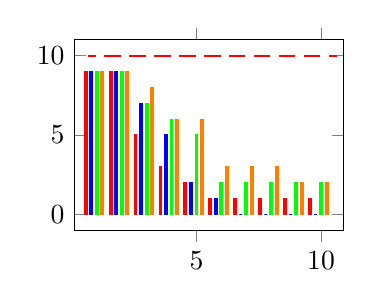
\begin{tikzpicture}
    \begin{axis}[
    width = 5cm,
    height=4cm,
    enlarge x limits = 0.1,
    enlarge y limits = 0.1,
    legend columns=1,
    ybar,
    bar width=1pt,
    ymin = 0,
    ymax = 10,
	compat=1.6,
	title={},
	%ylabel=goals 6,
]
\addplot+[ybar, bar shift =-4.0pt, red,
]
plot coordinates {
(03, 5) %c_125
(04, 3) %c_125
(05, 2) %c_125
(01, 9) %c_125
(02, 9) %c_125
(10, 1) %c_125
(08, 1) %c_125
(09, 1) %c_125
(06, 1) %c_125
(07, 1) %c_125
};
\label{plot:props_hff_bu_24}
\addplot+[ybar, bar shift =-2.0pt, blue,
]
plot coordinates {
(10, 0) %c_125
(04, 5) %c_125
(05, 2) %c_125
(01, 9) %c_125
(02, 9) %c_125
(08, 0) %c_125
(09, 0) %c_125
(03, 7) %c_125
(06, 1) %c_125
(07, 0) %c_125
};
\label{plot:props_hff_td_24}
\addplot+[ybar, bar shift =0.0pt, green,
]
plot coordinates {
(10, 2) %c_125
(04, 6) %c_125
(03, 7) %c_125
(01, 9) %c_125
(05, 5) %c_125
(02, 9) %c_125
(08, 2) %c_125
(09, 2) %c_125
(06, 2) %c_125
(07, 2) %c_125
};
\label{plot:props_trap_bu_24}
\addplot+[ybar, bar shift =2.0pt, orange,
]
plot coordinates {
(10, 2) %c_125
(04, 6) %c_125
(05, 6) %c_125
(01, 9) %c_125
(02, 9) %c_125
(08, 3) %c_125
(09, 2) %c_125
(03, 8) %c_125
(06, 3) %c_125
(07, 3) %c_125
};
\label{plot:props_trap_td_24}

%lmct
\addplot+[only marks, mark = -, mark options = {thick, red, dashed}, mark size = 0.2cm, black,
]
plot coordinates {
(02, 10)
(01, 10)
(04, 10)
(03, 10)
(07, 10)
(08, 10)
(06, 10)
(10, 10)
(05, 10)
(09, 10)
};
    \end{axis}
    \hfill
    
%\node[draw, align=center] (test) at (2,-2) {
%\ref{plot:props_hff_bu_24} hff-bu\\
%\ref{plot:props_hff_td_24} hff-td\\
%\ref{plot:props_trap_bu_24} trap-bu\\
%\ref{plot:props_trap_td_24} trap-td\\
%};

    \end{tikzpicture}
\end{minipage}
\begin{minipage}{0.22\textwidth}
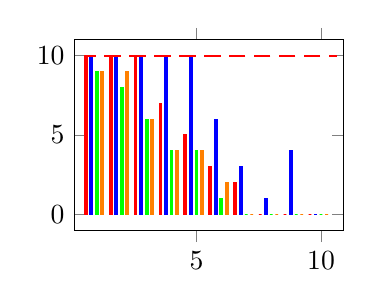
\begin{tikzpicture}
    \begin{axis}[
    width = 5cm,
    height=4cm,
    enlarge x limits = 0.1,
    enlarge y limits = 0.1,
    legend columns=1,
    ybar,
    bar width=1pt,
    ymin = 0,
    ymax = 10,
	compat=1.6,
	title={},
	%ylabel=goals 06,
]
\addplot+[ybar, bar shift =-4.0pt, red,
]
plot coordinates {
(07, 2) %c_125
(08, 0) %c_125
(03, 10) %c_125
(10, 0) %c_125
(06, 3) %c_125
(09, 0) %c_125
(02, 10) %c_125
(05, 5) %c_125
(04, 7) %c_125
(01, 10) %c_125
};
\label{plot:props_hff_bu_53}
\addplot+[ybar, bar shift =-2.0pt, blue,
]
plot coordinates {
(07, 3) %c_125
(08, 1) %c_125
(03, 10) %c_125
(10, 0) %c_125
(06, 6) %c_125
(09, 4) %c_125
(02, 10) %c_125
(05, 10) %c_125
(04, 10) %c_125
(01, 10) %c_125
};
\label{plot:props_hff_td_53}
\addplot+[ybar, bar shift =0.0pt, green,
]
plot coordinates {
(07, 0) %c_125
(08, 0) %c_125
(03, 6) %c_125
(10, 0) %c_125
(06, 1) %c_125
(09, 0) %c_125
(02, 8) %c_125
(05, 4) %c_125
(04, 4) %c_125
(01, 9) %c_125
};
\label{plot:props_trap_bu_53}
\addplot+[ybar, bar shift =2.0pt, orange,
]
plot coordinates {
(07, 0) %c_125
(08, 0) %c_125
(03, 6) %c_125
(10, 0) %c_125
(06, 2) %c_125
(09, 0) %c_125
(02, 9) %c_125
(05, 4) %c_125
(04, 4) %c_125
(01, 9) %c_125
};
\label{plot:props_trap_td_53}

%lmcut
\addplot+[only marks, mark = -, mark options = {thick, red, dashed}, mark size = 0.2cm, black,
]
plot coordinates {
(02, 10)
(01, 10)
(04, 10)
(03, 10)
(07, 10)
(08, 10)
(06, 10)
(10, 10)
(05, 10)
(09, 10)
};
    \end{axis}
    \hfill
    
%\node[draw, align=center] (test) at (2,-2) {
%\ref{plot:props_hff_bu_53} props-hff-bu\\
%\ref{plot:props_hff_td_53} props-hff-td\\
%\ref{plot:props_trap_bu_53} props-trap-bu\\
%\ref{plot:props_trap_td_53} props-trap-td\\
%};

    \end{tikzpicture}
\end{minipage}
\begin{minipage}{0.22\textwidth}
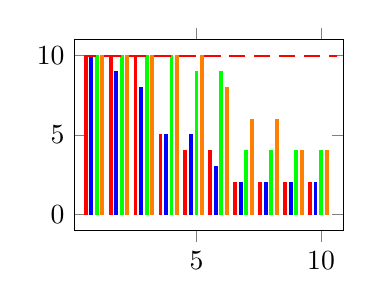
\begin{tikzpicture}

    \begin{axis}[
    width = 5cm,
    height=4cm,
    enlarge x limits = 0.1,
    enlarge y limits = 0.1,
    legend columns=1,
    ybar,
    bar width=1pt,
    ymin = 0,
    ymax = 10,
compat=1.6,
title={},
%ylabel=goals 7,
]
\addplot+[ybar, bar shift =-4.0pt, red,
]
plot coordinates {
(09, 2) %c_125
(05, 4) %c_125
(04, 5) %c_125
(07, 2) %c_125
(06, 4) %c_125
(10, 2) %c_125
(08, 2) %c_125
(03, 10) %c_125
(02, 10) %c_125
(01, 10) %c_125
};
\label{plot:props_hff_bu_68}
\addplot+[ybar, bar shift =-2.0pt, blue,
]
plot coordinates {
(09, 2) %c_125
(05, 5) %c_125
(04, 5) %c_125
(07, 2) %c_125
(06, 3) %c_125
(10, 2) %c_125
(08, 2) %c_125
(03, 8) %c_125
(02, 9) %c_125
(01, 10) %c_125
};
\label{plot:props_hff_td_68}
\addplot+[ybar, bar shift =0.0pt, green,
]
plot coordinates {
(09, 4) %c_125
(05, 9) %c_125
(04, 10) %c_125
(07, 4) %c_125
(06, 9) %c_125
(03, 10) %c_125
(08, 4) %c_125
(10, 4) %c_125
(02, 10) %c_125
(01, 10) %c_125
};
\label{plot:props_trap_bu_68}
\addplot+[ybar, bar shift =2.0pt, orange,
]
plot coordinates {
(09, 4) %c_125
(05, 10) %c_125
(04, 10) %c_125
(07, 6) %c_125
(06, 8) %c_125
(10, 4) %c_125
(08, 6) %c_125
(03, 10) %c_125
(02, 10) %c_125
(01, 10) %c_125
};
\label{plot:props_trap_td_68}

%lmcut
\addplot+[only marks, mark = -, mark options = {thick, red, dashed}, mark size = 0.2cm, black,
]
plot coordinates {
(02, 10)
(01, 10)
(04, 10)
(03, 10)
(07, 10)
(08, 10)
(06, 10)
(10, 10)
(05, 10)
(09, 10)
};
    \end{axis}
    \hfill
    
%\node[draw, align=center] (test) at (2,-2) {
%\ref{plot:props_hff_bu_68} props-hff-bu\\
%\ref{plot:props_hff_td_68} props-hff-td\\
%\ref{plot:props_trap_bu_68} props-trap-bu\\
%\ref{plot:props_trap_td_68} props-trap-td\\
%};

\end{tikzpicture}
\end{minipage}

